\documentclass{article}
\usepackage{parskip}
\usepackage{amsmath,amssymb,amsthm}
\usepackage{fullpage}
\usepackage{hyperref}
\usepackage{color}
\usepackage{graphicx}
\usepackage{mathpartir}

\newtheorem{thm}{Theorem}
\newtheorem{lemma}[thm]{Lemma}
\newtheorem{corollary}[thm]{Corollary}
\newtheorem{definition}[thm]{Definition}
\newtheorem{remark}[thm]{Remark}
\newtheorem{proposition}[thm]{Proposition}
\newtheorem{notn}[thm]{Notation}
\newtheorem{observation}[thm]{Observation}
\include{lam-ott}

\title{The $\lambda$-Calculus\\Programming Languages (CSCI 3300)\vspace{-22px}}
\author{Prof. Harley Eades (heades@gru.edu).}
\date{\vspace{-22px}}
\begin{document}
\maketitle  

In this lecture we are going to start to study our first functional
programming languages called the $\lambda$-Calculus.  This language
was first proposed by Alonzo Church in the early 1900's.  He was
studying the foundations of mathematics and thought it might be useful
for studying logic.  Later, he realized that it is a model of
computation.  That is, it is just as powerful as Turing Machines which
implies it is just as powerful as modern day computers.  In fact,
Turing Machines and the $\lambda$-calculus are equivalent.  This is
known as the Church-Turing thesis.  The thing that sets the
$\lambda$-calculus apart is that it is extermely simple.

Today the $\lambda$-calculus is as important as ever, and can be found
at the heart of all functional programming languages.  This includes
Haskell.  So when one is programming in Haskell they are programming
in the $\lambda$-calculus.

\section{The Language of the $\lambda$-Calculus}
\label{sec:the_lambda-calculus}
The $\lambda$-calculus is extermely simple.  In fact, it essentially
just consists of functions and function application.  The following
defines the grammar for the $\lambda$-calculus:
\begin{center}
  \begin{math}
    \begin{array}{rll}
      \text{(Variables)} & v ::= [[x]] \mid [[y]] \mid [[z]] \mid \ldots\\
      \text{(Terms)}     & t ::= [[v]] \mid [[\x.t]] \mid [[t1 t2]]\\
    \end{array}
  \end{math}
\end{center}
The language of the $\lambda$-calculus consists of an infinite number
of variables, anonymous unary functions, and function application.
That's all.

Variables are denoted $[[x]]$, $[[y]]$, and $[[z]]$.  We also
subscript variables to help distinguish them.  Keep in mind that there
are an infinite number of variable names, and we can name a variable
anything we wish.  However, it is common to stick to single letter
names with subscripts.  

\textbf{Variables are not the samething as variables in object
  oriented programming languages or imparative languages like C, C++,
  C\#, and Java.}  Variables in programming languages like those are
pointers to memeory, and can be reassigned multiple times.  However,
in the $\lambda$-calculus there is no memory.  One should think of the
variables in object oriented and imparative programming languages as
``assignables'' instead of variables, and think of the variables of
the $\lambda$-calculus as the variables one finds in mathematics.  The
variables in mathematics and the $\lambda$-calculus are
\textbf{replaced} with other objects and not assigned.  We will see
more of this replacment notion below.

Arguably the most important part of the $\lambda$-calculus is the
$\lambda$-abstraction (or anonymous unary function) denoted
$[[\x.t]]$.  We all $[[x]]$ the bound variable, and $[[t]]$ the body of
the $\lambda$-expression.  Here the variable $[[x]]$ is the
placeholder of the input to the function.  Keep in mind that the
argument variable -- here $[[x]]$ -- can be any variable at all.  It
does not have to always be called $[[x]]$. The best way to think of
these functions are as black boxes with only one input and one output:
\begin{center}
  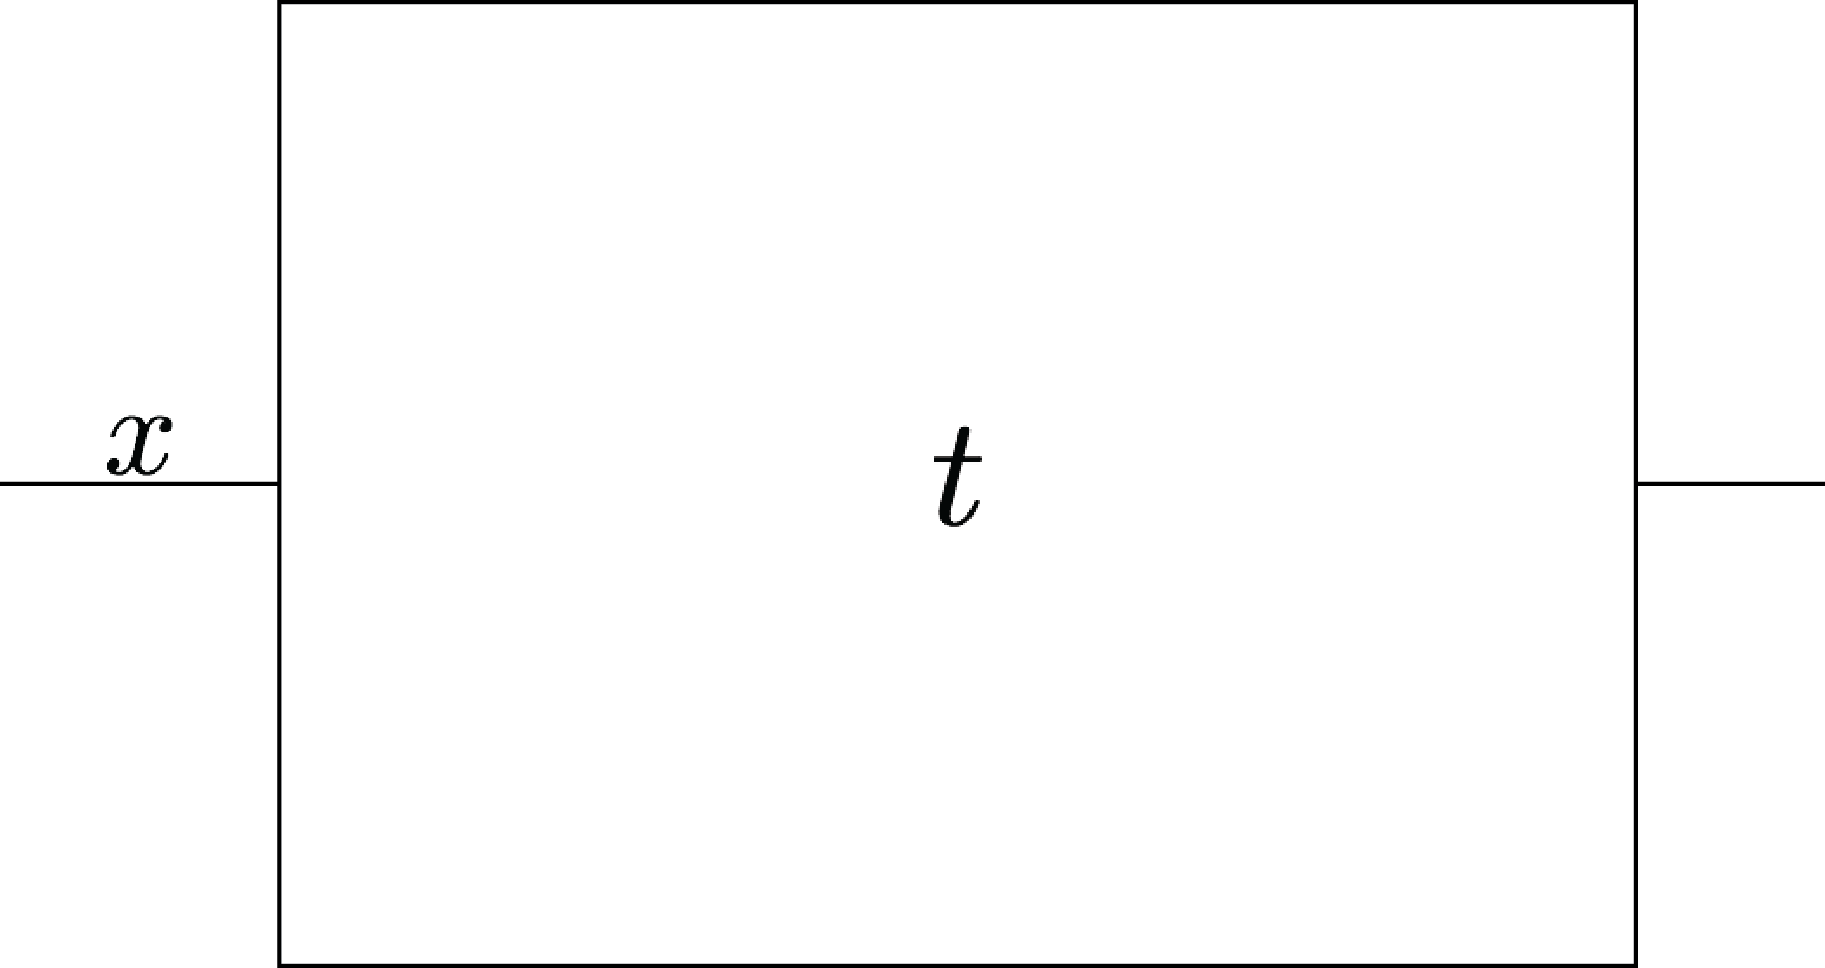
\includegraphics[scale=0.3]{black-blox}
\end{center}

The final piece of the language of the $\lambda$-calculus is function
application denoted $[[t1 t2]]$.  We will see that this is the locus
of computation.  Programs will be defined as functions, and running
programs will consist of simplifying function applications.  How this
simplifcation works will soon be discussed.  A note on terminology.
It is common to refer to terms as expressions and programs in general.
I will definately use this terms interchangeable.
% section the_$\lambda$-calculus (end)

\section{Example $\lambda$-Calculus Programs}
\label{sec:example_lambda-calculus_programs}
Here we give several example programs:
\begin{itemize}
\item The identity function: $[[\x.x]]$.
\item Forget the first $[[\x.\y.x]]$.
\item Forget the second $[[\x.\y.y]]$.
\item The successor function $[[\s.\x.h(s z)]]$.
\item Application: $[[(\x.x) y]]$.
\item Pairs: $[[\x.\y.\z.h((z x) y)]]$.
\item The first projection function: $[[\p.h(p (\x.\y.x))]]$.
\item The second projection function: $[[\p.h(p (\x.\y.y))]]$.
\end{itemize}
% section example_lambda-calculus_programs (end)

\section{Free and Bound Variables}
\label{sec:free-bound}

One of the more confusing notions to understand when it comes to
variables in the $\lambda$-calculus is their dual role.  In one
respect they can be seen as a global variable, while in another they
are to be considered as local variables.  

We call global variables ``free variables,'' and when we write
something like $[[y]]$ we call $[[y]]$ a free variable.  In addition,
the variables in $[[(x y) z]]$ are all free variables.  Similarly, the
variable $[[x]]$ in $[[\y.x]]$ is a free variable, but what about
$[[y]]$?

A variable whose name is the input to a function is called a ``bound
variable.''  For example, the variable $[[x]]$ is bound in $[[\x.x]]$.
A bound variable is a locally scoped one.  It is only useable from
within the body of its $\lambda$-abstraction.  Every variable in
$[[\x.h(\y.h(x y))]]$ is bound.  How about the rightmost $[[x]]$ in
$[[(\x.z) x]]$?  It is in fact, not bound, but free.  Note that for
some $\lambda$-abstraction $[[\x.t]]$ we say that $[[x]]$ is bound in
$[[t]]$, and we call the $\lambda x$ part the binder of the
$\lambda$-abstraction.  So in the previous example $[[(\x.z) x]]$ we
say that $[[x]]$ is bound in $[[z]]$, but the rightmost $[[x]]$ is
free in the entire term.

There is a pretty profound thing that occurs when we take a
$\lambda$-abstraction, say $[[\x.h(x y)]]$, and remove its binder to
obtain $[[x y]]$.  The variable $[[x]]$ changes from a bound variable
to a free variable.  That is, it changes from a locally scoped
variable to a globally scoped variable.  This may seem like a small
point, but when we start implementing programming languages with bound
variables this has profound implications.  It becomes not so easy to
implement.  We will see more of this later in the semester.
% section free_and_bound_variables (end)

\section{Parsing Conventions and Scope}
\label{sec:parsing_conventions}
We will be dealing with a lot of $\lambda$-expressions.  So it
convenient to have parsing conventions to make writing down
$\lambda$-expressions eaiser.  

First, $\lambda$-abstractions consume everything to the left of the
period, and this range also happens to be the scope of the input
variable.  So for example, consider the term $\lambda x.\lambda y.x\,z\,s\,s'$.
The parsing convention is that the body of the outter-most
$\lambda$-abstraction is $[[\y.h(h(h(x z) s) s')]]$.  That is it extends all
the way to the right most side of the expression.  This also happens
to be the scope of the input variable $[[x]]$.  So in $[[(\x.h(x y)) x]]$
the rightmost $[[x]]$ is not associated with the bound variable
$[[x]]$, in fact, these are two completely different variables -- the
first is bound while the second is free.  To prevent ambiguity with
scope use parentheses to delimit the bounds.  Reconsidering this term
$[[\x.h(\y.h(h(h(x z) s) s'))]]$ we can add parentheses to prevent ambiguity, that
is, $[[\x.(\y.(x z s s'))]]$ fully delimits the scope of each
$\lambda$-abstraction.

There is one other parsing convention that we will use.  Function
application associates to the left.  That is, the term $[[h(h(h(t1 t2)
t3) t4) t5]]$ is equivalent to $[[(((t1 t2) t3) t4) t5]]$.  

Now using these conventions we can fully parenthesize
$\lambda$-expressions to prevent ambiguity.  So the fully
parenthesized version of $[[\x.h(\y.h(\z.h(h(h(y z) x) w)))]]$ is
$[[\x.(\y.(\z.(((y z) x) w)))]]$.
% section parsing_conventions (end)

\section{Structural Recursion}
\label{sec:induction_and_recursion}
At this point we have only seen the language of the
$\lambda$-calculus, but this is supposed to be a programming language,
so how do we compute with these things?  Before we can answer that we
have to understand how we can define functions on the language of the
$\lambda$-calculus, and in order to do this we must understand
structural recursion.

Lets consider an example first.  Suppose we wanted to define a
function that operates on $\lambda$-calculus expressions (or simply
$\lambda$-expressions) that when given a $\lambda$-expression computes
its depth when considered as a tree.  How would we do this?  The following
accompishes this:
\begin{center}
  \begin{math}
    \begin{array}{rl}
      [[depth(x)]]    & = 1\\
      [[depth(\x.t)]] & = 1 + [[depth(t)]]\\
      [[depth(t1 t2)]] & = [[depth(t1)]] + [[depth(t2)]]      
    \end{array}
  \end{math}
\end{center}
The depth function takes a $\lambda$-expression as an arugment and
produces a number greater than or equal to $1$.  This function is
defined using the notion of \textbf{structural recursion}.  

Structural recursion is a device for defining functions over data that
is built up from smaller pieces of data.  For example, trees are built
up from smaller pieces of data.  We know a binary tree consists of a
leaf and a node that consists of two branches.  If we denote a leaf by
$\mathsf{leaf}\,n$ where $n$ can be any natural number, and we denote
nodes as $\mathsf{node}\,n\,T_1\,T_2$ where $T_1$ and $T_2$ are the
two child trees, then we can define any binary tree at all. An example
would be $\mathsf{node}\,1\,(\mathsf{node}\,2\, (\mathsf{leaf}\, 4)\,
(\mathsf{leaf}\, 5))\, (\mathsf{node}\, 3\, (\mathsf{leaf}\, 6)\,
(\mathsf{leaf}\, 7)))$.  This example in graphical form is:
\begin{center}
  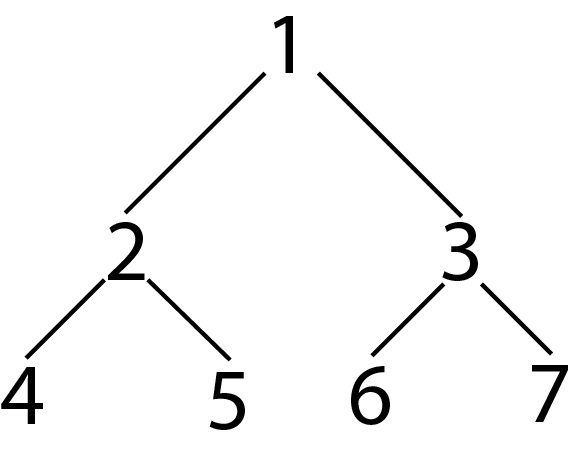
\includegraphics[scale=1]{tree-pieces}
\end{center}
Now trees have a clearly defined structure.  A leaf has no constituent
tree-parts, but a node has two constituent tree-parts: the left
subtree and the right subtree.  So using this idea we can define an
ordering on trees:
\begin{center}
  \begin{math}
    \begin{array}{lll}
      \mathsf{node}\,n\,T_1\,T_2 > T_1\\
      \mathsf{node}\,n\,T_1\,T_2 > T_2\\      
    \end{array}
  \end{math}
\end{center}
Notice that in the above definition we do not mention leafs and that
is because there is nothing smaller than a leaf.  The previous
ordering is the subtree ordering on binary trees.  

The idea that we are trying to get accross here is that any datatype
which can be built up from smaller pieces contains a natural
substructure ordering.  This can then be used to define functions by
recursion.  Remember, a recursive function has at least one base case,
and at least one step case.  For the case of trees, the base case
would be for leafs, and the step case would be for nodes.  Similarly,
for the case of $\lambda$-expressions the base case is for variables,
and the step case is for $\lambda$-abstractions and application.  Then
we are allowed to make recursive calls on the subdata whether it be a
subtree or a sub-$\lambda$-expression.  

Lets consider an example function defined by structural recursion on
trees.  The following computes the set of tree data given any tree:
\begin{center}
  \begin{math}
    \begin{array}{rll}
      \mathsf{flatten}(\mathsf{leaf}\,n) & = \{ n \}\\
      \mathsf{flatten}(\mathsf{node}\,m\,T_1\,T_2) & = \{m\} \cup \mathsf{flatten}(T_1) \cup \mathsf{flatten}(T_2)\\
    \end{array}
  \end{math}
\end{center}
Now flattening our example tree from above we obtain:
\begin{center}
  \begin{math}
    \begin{array}{lll}
      \mathsf{flatten}(\mathsf{node}\,1\,(\mathsf{node}\,2\, (\mathsf{leaf}\, 4)\,
      (\mathsf{leaf}\, 5))\, (\mathsf{node}\, 3\, (\mathsf{leaf}\, 6)\,
      (\mathsf{leaf}\, 7))) \\
      \,\,\,\,\,\,\,= \{1\} \cup \mathsf{flatten}(\mathsf{node}\,2\, (\mathsf{leaf}\, 4)\,
      (\mathsf{leaf}\, 5)) \cup \mathsf{flatten}(\mathsf{node}\, 3\, (\mathsf{leaf}\, 6)\,
      (\mathsf{leaf}\, 7))\\
      \,\,\,\,\,\,\,= \{1\} \cup \{2\} \cup \mathsf{flatten}(\mathsf{leaf}\, 4) \cup \mathsf{flatten}(\mathsf{leaf}\, 5) \cup \mathsf{flatten}(\mathsf{node}\, 3\, (\mathsf{leaf}\, 6)\,
      (\mathsf{leaf}\, 7))\\
      \,\,\,\,\,\,\,= \{1\} \cup \{2\} \cup \mathsf{flatten}(\mathsf{leaf}\, 4) \cup \mathsf{flatten}(\mathsf{leaf}\, 5) \cup \{3\} \cup \mathsf{flatten}(\mathsf{leaf}\, 6) \cup \mathsf{flatten}(\mathsf{leaf}\, 7)\\
      \,\,\,\,\,\,\,= \{1\} \cup \{2\} \cup \{4\} \cup \mathsf{flatten}(\mathsf{leaf}\, 5) \cup \{3\} \cup \mathsf{flatten}(\mathsf{leaf}\, 6) \cup \mathsf{flatten}(\mathsf{leaf}\, 7)\\
      \,\,\,\,\,\,\,= \{1\} \cup \{2\} \cup \{4\} \cup \{5\} \cup \{3\} \cup \mathsf{flatten}(\mathsf{leaf}\, 6) \cup \mathsf{flatten}(\mathsf{leaf}\, 7)\\
      \,\,\,\,\,\,\,= \{1\} \cup \{2\} \cup \{4\} \cup \{5\} \cup \{3\} \cup \{6\} \cup \mathsf{flatten}(\mathsf{leaf}\, 7)\\
      \,\,\,\,\,\,\,= \{1\} \cup \{2\} \cup \{4\} \cup \{5\} \cup \{3\} \cup \{6\} \cup \{7\}\\
      \,\,\,\,\,\,\,= \{1, 2, 4, 5, 3, 6, 7\}\\
    \end{array}
  \end{math}
\end{center}

Getting back to the $\lambda$-calculus we can now use structural
recursion to define functions over $\lambda$-expressions just like the
depth function from above.  In fact, just as we saw for trees there is
a natural structural ordering on $\lambda$-expressions:
\begin{center}
  \begin{math}
    \begin{array}{lll}
      [[\x.t]] > [[t]]\\
      [[t1 t2]] > [[t1]]\\
      [[t1 t2]] > [[t2]]\\
    \end{array}
  \end{math}
\end{center}
Again, variables are the base case, so they do not appear in the above
definition.  Now notice that the above ordering is terminating, that
is, given an arbitrary term, it can only get smaller for a finite
amount of time.  That is, eventually we must bottom out at a variable.
The fact that this ordering must terminate impilies that the
depth function from above must always produce an output. 

Functions defined on languages like the $\lambda$-expressions are
known as metafunctions, because they can be thought of as living
outside the actually language.  We will see a number of these
throughout the semester.
% section recursion (end)

\section{Variable Substitution}
\label{sec:variable_substitution}
I mentioned above that a variables job is to be replaced by other
$\lambda$-expressions.  At this point we define how this replacement
is done, and then use this new definition to define how to compute
with $\lambda$-expressions.

The substitution meta-function on $\lambda$-expressions is defined as follows:
\begin{center}
  \begin{math}
    \begin{array}{lll}
      [[ [t/x]x ]] = [[t]]\\
      & \\
      [[ [t/x]y ]] = [[y]]\\
      \,\,\,\,\,\text{ where } [[y]] \text{ is distinct from } [[x]]\\
      & \\
      [[ [t/x](\y.t') ]] = [[\y.[t/x]t']]\\
      \,\,\,\,\,\,\text{ where } [[y]] \text{ is distinct from } [[x]]\\
      & \\
      [[ [t/x](\x.t') ]] = [[\x.t']]\\
      & \\
      [[ [t/x](t1 t2) ]] = [[([t/x]t1) ([t/x]t2)]]
    \end{array}
  \end{math}
\end{center}
The substitution function denoted $[[ [t/x]t' ]]$ takes in three
arguments: $[[t]]$, $[[x]]$, and $[[t']]$.  We read it as ``substitute
$[[t]]$ for $[[x]]$ in $[[t']]$.''  Intuitively, we can think of it as
simply replacing every occurrence of $[[x]]$ with $[[t]]$ in $[[t']]$.
However, one has to be careful to not replace a bound variable.  The
second and third conditions in the above definition prevent this from
happening.  In Section~\ref{sec:free-bound} we discussed the
difference between bound variables and free variables.  \textbf{We are
  only allowed to replace free variables using substitution.}

Some examples:
\begin{itemize}
\item $[[ [y/x]x ]] = [[y]]$
\item $[[ [y/x]z ]] = [[z]]$ where $[[z]]$ is distinct from $[[x]]$
\item $[[ [y/z](\x.z)]] = [[\x.[y/z]z]] = [[\x.y]]$
\item $[[ [y/z]((\x.x) z) ]] = [[([y/z](\x.x)) ([y/z]z)]] = [[(\x.[y/z]x) ([y/z]z)]] = [[(\x.x) y]]$
\item $[[ [\x.\y.y/z] ((z s) s')]] = [[ ([\x.\y.y/z] (z s)) ([\x.\y.y/z] s')]]$\\ 
  $      \,\,\,\,\,\,\,\,\,\,\,\,= [[ (([\x.\y.y/z] z) ([\x.\y.y/z] s)) ([\x.\y.y/z] s')]]$\\
  $ = [[ ((\x.\y.y) s) s']]$
\end{itemize}
% section variable_substitution (end)

\section{Inference Systems}
\label{sec:inference_rules}

A lot of the design of programming languages in general involve the
careful definition of certain algorithms that manipulate programs.
This is similar to the idea of defining functions on programs like the
$\mathsf{depth}$ function we saw in class.  A large number of
algorithms can be described using inference systems.

An inference system consists of one or more inference rules.  An
inference rule has the following shape:
\begin{center}
  \begin{math}
    $$\mprset{flushleft}
    \inferrule* [right=Name] {
      P_1
      \\
      \cdots
      \\
      P_n
    }{C}
  \end{math}
\end{center}
We call $P_1, \cdots, P_n$ the premises of the rule, and $C$ the
conclusion.  Note that it is completely satisfactory to have an
inference rule with no premises at all. In fact, an inference rules
with no premises are called axioms. Inference rules are read from the
top down as an if-statement.  So the above rule should be read "If
$P_1$, $P_2$, $\ldots$, and $P_n$ all hold, then $C$ holds."  If an
inference rule has no premises at all, then its conclusion always
holds, hence, the term axiom.  

An example may help.  The following set of inference rules define what
it means to be a binary tree:
\begin{center}
  \begin{math}
    \begin{array}{cc}
      $$\mprset{flushleft}
      \inferrule* [right=leaf] {
        n \in \mathbb{N}
      }{(\mathsf{leaf}\,n)\,Tree}
      &
      $$\mprset{flushleft}
      \inferrule* [right=node] {
        T_1\,Tree
        \\
        T_2\,Tree
        \\
        n \in \mathbb{N}
      }{(\mathsf{node}\,n\,T_1\,T_2)\,Tree}
    \end{array}
  \end{math}
\end{center}
The first rule states, "for all $n \in \mathbb{N}$, $\mathsf{leaf}\,n$
is a tree." Now the second states that "for any $T_1$, $T_2$, and $n
\in \mathbb{N}$, if $T_1$ and $T_2$ are trees, then
$\mathsf{node}\,n\,T_1\,T_2$ is a tree."

So what are these rules good for?  Inference system should be thought
of as an algorithm where the conclusion, $C$, is an input, and the
output essentially amounts to yes or no.  The former indicating that
the input adheres to the rules, and no otherwise.  So for example,
given the rules above we can ask is
$\mathsf{node}\,1\,(\mathsf{node}\,2\, (\mathsf{leaf}\, 4)\,
(\mathsf{leaf}\, 5))\, (\mathsf{node}\, 3\, (\mathsf{leaf}\, 6)\,
(\mathsf{leaf}\, 7))$ a tree, but how can we actually answer this
question?  We answer this question by building derivations of the
rules.  This is all very similar to how we used grammars.

A derivation is the application of one or more rules.  For example,
one of the simplest derivations using the rules for trees is the
following:
\begin{center}
  \begin{math}
    $$\mprset{flushleft}
    \inferrule* [right=leaf] {
      1 \in \mathbb{N}
    }{(\mathsf{leaf}\,1)\,Tree}
  \end{math}
\end{center}
In the above $\mathsf{leaf}\,1$ is the input, and the derivation
consists of only the rule $\mathtt{leaf}$, and this successfully shows
that $\mathsf{leaf}\,1$ is indeed a tree.  A more complete derivation
is the follows:
  \begin{center}
    \scriptsize
    \begin{math}
      $$\mprset{flushleft}
    \inferrule* [right=\scriptsize node] {
      $$\mprset{flushleft}
      \inferrule* [right=\scriptsize node] {
        $$\mprset{flushleft}
        \inferrule* [right=\scriptsize leaf] {
          4 \in \mathbb{N}
        }{(\mathsf{leaf}\, 4)\,Tree}
        \\
        $$\mprset{flushleft}
        \inferrule* [right=\scriptsize leaf] {
          5 \in \mathbb{N}
        }{(\mathsf{leaf}\,5)\,Tree}
        \\
        2 \in \mathbb{N}
      }{(\mathsf{node}\,2\, (\mathsf{leaf}\, 4)\,(\mathsf{leaf}\, 5))\,Tree}
      \\
      $$\mprset{flushleft}
      \inferrule* [right=\scriptsize node] {                
        $$\mprset{flushleft}
        \inferrule* [right=\scriptsize leaf] {
          6 \in \mathbb{N}
        }{(\mathsf{leaf}\, 6)\,Tree}
        \\
        $$\mprset{flushleft}
        \inferrule* [right=\scriptsize leaf] {
          7 \in \mathbb{N}
        }{(\mathsf{leaf}\, 7)\,Tree}
        \\
        3 \in \mathbb{N}
      }{(\mathsf{node}\, 3\, (\mathsf{leaf}\, 6)\,(\mathsf{leaf}\, 7))\,Tree}
      \\
      1 \in \mathbb{N}
    }{(\mathsf{node}\,1\,(\mathsf{node}\,2\, (\mathsf{leaf}\, 4)\, (\mathsf{leaf}\, 5))\, (\mathsf{node}\, 3\, (\mathsf{leaf}\, 6)\,(\mathsf{leaf}\, 7)))\,Tree}
    \end{math}
  \end{center}
  Derivations are constructed from the bottom up.  In the above we
  begin by asking the question, ``does
  $(\mathsf{node}\,1\,(\mathsf{node}\,2\, (\mathsf{leaf}\, 4)\,
  (\mathsf{leaf}\, 5))\, (\mathsf{node}\, 3\, (\mathsf{leaf}\,
  6)\,(\mathsf{leaf}\, 7)))\,Tree$ hold?''  To prove that it holds we
  try to apply the rules of the tree inference system one at a time,
  from the bottom up.  So after asking the question we try and pattern
  match on the conclusion of each rule.  If what we are asking matches
  the conclusion of the rule, then we may then move to the premises of
  that rule.  For example, we construct the above derivation by
  starting like this, we first asking the question:
  \begin{center}
    \begin{math}
      (\mathsf{node}\,1\,(\mathsf{node}\,2\, (\mathsf{leaf}\, 4)\, (\mathsf{leaf}\, 5))\, (\mathsf{node}\, 3\, (\mathsf{leaf}\, 6)\,(\mathsf{leaf}\, 7)))\,Tree
    \end{math}
  \end{center}
  Then we try to pattern match on the previous statement against the
  conclusion of each rule, and we can see that it matches the
  conclusion of the $\mathtt{node}$ rule, where $n = 1$, $T_1 =
  (\mathsf{node}\,2\, (\mathsf{leaf}\, 4)\, (\mathsf{leaf}\, 5))$, and
  $T_2 = (\mathsf{node}\, 3\, (\mathsf{leaf}\, 6)\,(\mathsf{leaf}\,
  7))$.  So we are allowed to apply that rule:
    \begin{center}
    \scriptsize
    \begin{math}
      $$\mprset{flushleft}
      \inferrule* [right=\scriptsize node] {
        (\mathsf{node}\,2\, (\mathsf{leaf}\, 4)\,(\mathsf{leaf}\, 5))\,Tree
        \\
        (\mathsf{node}\, 3\, (\mathsf{leaf}\, 6)\,(\mathsf{leaf}\, 7))\,Tree
        \\
        1 \in \mathbb{N}
      }{(\mathsf{node}\,1\,(\mathsf{node}\,2\, (\mathsf{leaf}\, 4)\, (\mathsf{leaf}\, 5))\, (\mathsf{node}\, 3\, (\mathsf{leaf}\, 6)\,(\mathsf{leaf}\, 7)))\,Tree}
    \end{math}
  \end{center}
  Then we ask, which rule can be applied to each premise?  Then we
  proceed until no further rules can be applied.  Eventually we end up
  with the derivation from above.

  Now how do we know when a derivation is successful?  First, notice
  that the derivations are themselves tree structures. The axioms are
  the leaves of the tree, and the premises start branches of the tree.
  For example, in the above example of the complete derivation using
  the tree inference system we can see that the $\mathtt{node}$ rule
  forms two branches, one for each subtree.  Now a derivation is
  \textbf{successful} if and only if every branch of the derivation
  ends in an axiom.  That is, the very last rules on the top of the
  derivation must be all axioms.  If not, then the derivation is a
  failure, and the conclusion is said not to hold.  The following is
  an example of a failure:
  \begin{center}
    \begin{math}
      $$\mprset{flushleft}
      \inferrule* [right=node] {
        $$\mprset{flushleft}
        \inferrule* [right=leaf] {
          2 \in \mathbb{N}
        }{(\mathsf{leaf}\,2)\,Tree}
        \\
        42
        \\
        1 \in \mathbb{N}
      }{(\mathsf{node}\,1\,(\mathsf{leaf}\,2)\,42)\,Tree}
    \end{math}
  \end{center}
  The previous derivation fails, because there is no rule to apply
  $42$ to and thus the derivation does not end in all axioms -- that
  is the $\mathtt{leaf}$ rule.  Therefore, we must conclude that
  $\mathsf{node}\,1\,(\mathsf{leaf}\,2)\,42$ is not a valid tree.  

  Inference systems usually have a particular goal called a judgment.
  The inference system is said to judge whether not something is
  provable or not.  For example, the tree inference system judges
  whether or not some mathematical object is a tree, and we can read
  the judgement $t\,Tree$ as ``$t$ is a tree.''  We then say that a
  judgment holds or is provable or is derivable if and only if we can
  construct a successful derivation of it.

  Inference systems are everywhere in programming language design.
  They allow for a very nice, compact, and easy definitions of
  algorithms on the objects of a programming language. Now we can use
  inference systems to define how we can compute in the
  $\lambda$-calculus.
% section inference_rules (end)

\section{Computing in the $\lambda$-Calculus}
\label{sec:computing_in_the_lambda-calculus}

The locus of computation in the $\lambda$-calculus is function
application, $[[t1 t2]]$, but even more specifically it is the
application of a $\lambda$-abstraction to an argument, that is,
$[[(\x.t) t']]$.  It turns out that computation in the
$\lambda$-calculus is really just a matter of replacing every
occurrence of $[[x]]$ in $[[t]]$ with $[[t']]$, but how do we do this
formally?  We use an inference system:
\begin{center}
  \begin{math}
    \begin{array}{cc}
      \ottdruleBeta{} &      \ottdruleLam{}  \\
      & \\
      \ottdruleAppOne{} &       \ottdruleAppTwo{}\\
    \end{array}
  \end{math}
\end{center}
The judgment here is $[[t1]] \rightsquigarrow [[t2]]$ which can be
read as $[[t1]]$ reduces to $[[t2]]$.  We call this set of inference
rules the reduction rules for the $\lambda$-calculus.  Note that one
should think of the terms in these rules as schemas of terms that we
match pattern against.  So some care has to be taken when checking to
see if a rule applies.  The reduction rules should be used just as we
used the tree inference system above.  That is, we begin with a
judgment that looks like $[[t1 ~> t2]]$, and then try to prove that
$[[t1]]$ reduces to $[[t2]]$ if we can construct a successful
derivation of $[[t1 ~> t2]]$ using the reduction rules.  We can think
of this style as starting with some solution to a problem, and then
using the rules to check to see if the solution is correct.

The most important rule is the $\beta$-rule:
\[\ottdruleBeta{} \]
This rule says that any term matching the pattern $[[(\x.t) t']]$ can
be replaced by $[t'/x]t$ which replaces every occurrence of $[[x]]$
with $[[t']]$ in $[[t]]$. 
\vspace{10px}
\begin{definition}[Redex]
  \label{def:redex}
  Any term matching $[[(\x.t) t']]$ is called a \textbf{redex}.
\end{definition}
So we can see that the term in the lefthand side of the arrow in the
$\beta$-rule is the redex, and we call the righthand side the
\textbf{contractum}.  Notice that variable substitution is an
important part of the $\beta$-rule, and now we can see that computing
really amounts to using the $\beta$-rule which amounts to just using
the variable substitution function to simplify function applications.

Now lets consider an example using the $\beta$-rules.  The following shows
that $[[(\x.x) y]]$ reduces to $y$.
\begin{center}
  \begin{math}
    $$\mprset{flushleft}
    \inferrule* [right=Beta] {
      \,
    }{[[(\x.x) y ~> y]]}
  \end{math}
\end{center}
This holds because the term $[[(\x.x) y]]$ matches the pattern
$[[(\x.t) t']]$ where the binder $[[x]]$ is $[[x]]$, $[[t]]$ is
$[[x]]$, and $[[t']]$ is $[[t]]$, and $[[ [y/x]x ]] = [[y]]$.  So
sometimes this rule is hard to apply because we have to reverse the
substitution function, that is, we had to realize the $[[y]]$ is the
same as $[[ [y/x]x]]$ when just given $[[y]]$.

The reduction rules are literal.  One can only apply the rule if the
terms given match the term patterns in the conclusion.  For example,
can we apply the $\beta$-rule to conclude $[[x ((\y.h(y z)) r) ~> x (r
z)]]$?  No, because $[[x ((\y.h(y z)) r)]]$ does not match the pattern
$[[(\x.t) t']]$, and $[[x (r z)]]$ does not match the pattern $[[
[t'/x]t]]$ so that rule does not apply, but we should be allowed to
reduce that redex, right?  This is the job for the other reduction
rules.


There are three other reduction rules:
\begin{center}
  \begin{math}
    \begin{array}{lll}
      \ottdruleLam{}  & \ottdruleAppOne{} \\
      & \\
      \ottdruleAppTwo{}\\
    \end{array}
  \end{math}
\end{center}
These rules allow us to move inside of terms.  For example, we can
now show $[[x ((\y.h(y z)) r) ~> x (r z)]]$:
\begin{center}
  \begin{math}
    $$\mprset{flushleft}
    \inferrule* [right=App2] {
      $$\mprset{flushleft}
      \inferrule* [right=Beta] {
        \,
      }{[[(\y.h(y z)) r ~> (r z)]]}
    }{[[x ((\y.h(y z)) r) ~> x (r z)]]}
  \end{math}
\end{center}

Consider this term for example, $[[(\x.h(x x))((\y.y) r)]]$, how many
redexes are there in this term? There are two, the entier term, and
the subterm $[[(\y.y) r]]$.  So how do we reduce them both?  In fact,
we cannot do this, because these rules only support reducing exactly
one redex.  In fact, the reduction rules we have considered so far are
called the \textbf{single-step full $\beta$-reduction.}  The ``full''
part has to do with the ability to contract a redex anywhere within a
term.

To allow for the reduction of multiple redexes we define a new
inference system called \textbf{multi-step full $\beta$-reduction.}
The inference system is as follows:
\begin{center}
  \begin{math}
    \begin{array}{lll}
     \ottdruleRefl{} & \ottdruleSStep{} & \ottdruleMStep{}
    \end{array}
  \end{math}
\end{center}

Now we can use this inference system to reduce more than one redex at a time.
For example we can prove the following reductions (full derivations in class):
\begin{center}
  \begin{math}
    \begin{array}{lll}
      [[h(x ((\y.y)((\z.h(z z)) r))) ~*> x (r r)]] \\
      [[\y.h((\x.\y.y)((\x.h(x x))(\x.h(x x))) z) ~*> \y.z]]
    \end{array}
  \end{math}
\end{center}

There is one downfall of applying the reduction rules the way that we
have.  The redex is often the program the programmer has written, and
the contractum is either the solution, or an intermediate point to the
solution.  So from here on out we -- unless directed differently like
in homeworks or exams -- we are going to adopted a different way of
applying these rules.  We will use these rules a guiding principle for
how to transform a term into another by contracting its redexes.  So
instead of writing down long and big derivations we will simply write
down a chain of transformations.  These transformations a very similar
to the derivations we did on grammars.  Lets consider an example.
\begin{center}
  \begin{math}
    \begin{array}{lll}
      [[ul((\n.h(\m.(\s.h(\z.h((n s) (m s z)))))) (\s.h(\z.h(s z))) (\s.h(\z.h(s (s z)))))]] \\
      \,\,\,\,\,\,\,\,\,\,\rightsquigarrow [[ul((\m.(\s.h(\z.h(((\s.h(\z.h(h(s z) s))) (m s z)))))) (\s.h(\z.h(s (s z)))))]]\\
      \,\,\,\,\,\,\,\,\,\,\rightsquigarrow [[\s.h(\z.h((((\s.h(\z.h(h(s z)))) s) ul(((\s.h(\z.h(s (s z)))) s z)))))]]\\
      \,\,\,\,\,\,\,\,\,\,\rightsquigarrow [[\s.h(\z.h((ul(((\s.h(\z.h(h(s z)))) s)) (s (s z)))))]]\\
      \,\,\,\,\,\,\,\,\,\,\rightsquigarrow [[\s.h(\z.ul(h((\z.h(s z)) (s (s z)))))]]\\
      \,\,\,\,\,\,\,\,\,\,\rightsquigarrow [[\s.h(\z.h(s (s (s z))))]]\\
    \end{array}
  \end{math}
\end{center}
Notice how in the above I underlined the redex I was contracting in
each step.  This is required when writing these down in your homework
and exams, because it makes it apparent which redex we are contracting
at each step.  Also, notice that where we can put the underline is
determined by the rule of the inference system.  Lastly, each
transformation is step in the single-step full $\beta$-reduction
inference system.  However, if one can give a chain of one or more
transformations from $[[t1]]$ to $[[t2]]$, then we can derive $[[t1
~*> t2]]$ in the multi-step full $\beta$-reduction inference system.
% section computing_in_the_lambda-calculus (end)

% \section{Reduction Order}
% \label{sec:reduction_order}
% The reduction rules for the $\lambda$-calculus do not enforce any
% particular order of reduction.  That is, we can choose to contract any
% redex we wish.  This does have an important consequence. Consider the
% following $\lambda$-expression:
% \[ [[h((\x.\y.x) z) ((\x.h(x x)) (\x.h(x x)))]] \] Suppose we choose
% to always reduce the second argument, then the previous expression
% will run forever.  Now suppose that we always choose to reduce the
% left-most redex, then we will obtain the following reduction sequence:
% \begin{center}
%   \begin{math}
%     \begin{array}{lll}
%       [[h((\x.\y.x) z) ((\x.h(x x)) (\x.h(x x)))]] & \redto & [[h(\y.z) ((\x.h(x x)) (\x.h(x x)))]]\\
%       & \redto & [[z]]\\
%     \end{array}
%   \end{math}
% \end{center}
% This example shows that the reduction order has a pretty dramatic
% effect.  It can determine whether or not a program terminates!
% % section reduction_order (end)

% \section{Termination}
% \label{sec:termination}
% The $\lambda$-calculus is the craziest of crazy programming languages.
% You can write terminating programs as well as non-terminating
% programs.  For example, the over used $\lambda$-expression called
% $\Omega$ is defined as $[[(\x.h(x x))(\x.h(x x))]]$.  This clearly
% does not terminate.  In the previous section we saw that depending on
% which redex one chooses to reduce a program may terminate or diverge
% -- never terminate.  Is it possible to give a reduction order -- a
% specific ordering on which redex to choose -- that will guarantee that
% if a program terminates, then it will?

% It turns out that we can, and the reduction order is called
% normal-order reduction.  The rule is that one must \textbf{always}
% reduce the left-most outer-most redex in a $\lambda$-expression.  If
% one does this, and the $\lambda$-expression being reduced can
% terminate, then normal-order reduction will terminate.
% % section termination (end)

% \section{Normal-Order Reduction}
% \label{sec:normal-order_reduction}
% In this section we modify the definition of the $\lambda$-calculus to
% restrict the reduction to normal-order only.   To do this we introduce
% a new concept called a evaluation contexts.  These are simply a
% different presentation of the rules we have now.  

% Before defining normal-order reduction lets first redefine full
% $\beta$-reduction using evaluation contexts.  The syntax of the
% $\lambda$-calculus is redefined as follows:
% \begin{center}
%   \begin{math}
%     \begin{array}{lll}
%       \text{(Terms)}    & [[t]] ::= [[x]] \mid [[\x.t]] \mid [[t1 t2]]\\
%       \text{(Contexts)} & [[C]] ::= [[*]] \mid [[\x.C]] \mid [[t C]] \mid [[C t]]\\
%     \end{array}
%   \end{math}
% \end{center}
% We call $[[*]]$ the hole.  So a context $[[C]]$ is a $\lambda$-term
% with a hole in it.  Notice that we can only have one hole.  This is
% key.  The hole denotes the location of where the redex we are going to
% contact resides.  We denote filling this hole, that is replacing
% $[[*]]$ in a context $[[C]]$ with a term $[[t]]$, by $[[C[t] ]]$. Suppose our context $[[C]]$ is $[[\x.h(z *)]]$, then, $[[C[ \y.h(y y)] ]] = [[(\x.h(z *))[\y.h(y y)] ]] = [[\x.h(z (\y.h(y y)))]]$.  We can see that we simply just replaced (plugged) the
% $[[*]]$ (the hole) with $[[\y.h(y y)]]$.  In addition, the context
% $[[C]]$ encapsulates the term around the hole or where the redex
% resides.  So contexts formally define ``ripping out the redex'' as I
% have been saying during lecture.

% Now using evaluation contexts we can collapse all of our inference
% rules into one rule only:
% \begin{center}
%   \begin{math}
%     $$\mprset{flushleft}
%     \inferrule* [right=Beta] {
%       \,
%     }{[[C[(\x.t) t'] ]] \redto [[C[ [t'/x]t] ]]}
%   \end{math}
% \end{center}
% The congurence rules are encoded into the context, because we can
% contract any redex where a hole is located in an evaluation context.
% So for example,
% \begin{center}
%   \begin{math}
%     \begin{array}{lll}
%       EXAMPLE
%     \end{array}
%   \end{math}
% \end{center}
% % section normal-order_reduction (end)

% \bibliographystyle{plain}
% \bibliography{thesis}
\end{document}
